\documentclass{article} % PDFTex, XeLaTex 都支持。

% 中文环境
%\documentclass[hyperref, UTF8]{ctexart} %若选择{ctexart}则直接支持中文,下面的{ctex}要去掉。
%\usepackage[UTF8]{ctex} %中文配置。
%\usepackage[UTF8, heading=false, scheme=plain]{ctex} %加入scheme=plain,行距、中西文公共字符都有变化。

% 版面设置
\usepackage{geometry}
\geometry{a4paper}

% 额外的功能
\usepackage{authblk} %添加机构,需要安装preprint包
\usepackage{amsthm} %证明环境
\usepackage{amsmath} %数学公式
\numberwithin{equation}{section} % 公式按章节编号
\usepackage{amssymb}
\usepackage{multirow} % multirow
\usepackage{booktabs} % toprule, midrule, bottomrule

% 表格的单元格内换行、对齐功能
\usepackage{makecell}

% 图片支持
\usepackage{graphicx} %添加图片
\graphicspath{{figures/}}
\usepackage{float} % 控制图片是否浮动:[htbp]浮动,或[H]禁止浮动

% PDF索引及超链接 (black,red,blue,green)
\usepackage[colorlinks=true,linkcolor=black,anchorcolor=black,citecolor=blue,filecolor=black,menucolor=black,runcolor=black,urlcolor=black]{hyperref}

% 首行缩进
\usepackage{indentfirst} % 首行缩进支持
\setlength{\parindent}{2em} % 首行缩进两个汉字

% 列表样式定制
\usepackage{enumerate}
\usepackage{enumitem}
\setlist[enumerate,1]{label=(\arabic*).,font=\textup,leftmargin=14mm,labelsep=1.5mm,topsep=0mm,itemsep=-0.8mm}
\setlist[enumerate,2]{label=(\alph*).,font=\textup,leftmargin=14mm,labelsep=1.5mm,topsep=-0.8mm,itemsep=-0.8mm}
%\setlist{nosep} % 取消行间空行

% 自定义命令
\newcommand{\SL}{\rule{.3em}{.3pt}} % 定义短下划线

% 名称、作者、机构
\title{Formal Method Library for Flight Control System in Coq}
\author{Zhengpu Shi}
\affil{Draft V1.0}
%\affil{南京航空航天大学}
\date{Jan 01, 2021} %注释后显示为编译时日期


\begin{document}

% 生成标题
\maketitle
%\newpage
% ++++++++++++++++++++++++++++++++++++++++++++++++++++++++++++++++++++++++++++++++++++++++++++++++++

% 生成目录
%\tableofcontents
%\newpage
% ++++++++++++++++++++++++++++++++++++++++++++++++++++++++++++++++++++++++++++++++++++++++++++++++++

%\listoffigures
%\newpage
% 生成图片列表,请删除上面两行注释

%\begin{figure}[H]%[htbp]
%\centering\includegraphics[scale=0.85]{graph.jpg}
%\centerline{\includegraphics[width=1.0\textwidth]{graph.jpg}}
%\caption{this is a figure demo}
%\label{fig:label}
%\end{figure}

%\newpage
% ++++++++++++++++++++++++++++++++++++++++++++++++++++++++++++++++++++++++++++++++++++++++++++++++++
%\section*{摘要}


%\newpage
% ++++++++++++++++++++++++++++++++++++++++++++++++++++++++++++++++++++++++++++++++++++++++++++++++++

\section{Intorduction}
Aircraft is a big category of products in the Safety Critical Areas, including aircraft, spacecraft, guided weapons and so on.
The aircraft can operate semi-autonomously or fully autonomously, and they all need to be equipped with flight control software (FCS) to control their operations.
FCS is a highly complex software product with high reliability requirements.
Although a lot of manpower and material resources have been invested in the research and development of FCS, flight faults caused by software errors often occur.
%可以分段
Existing software development methods cannot completely eliminate software defects, for at least three possible reasons.
First, software programming models derived from flight control theory may contain errors.
Because lots of manual derivation.
Second, the process of converting the FCS model into FCS program may have errors.
Becuaes lots of manual coding.
Third, traditional software testing methods havn't ability to prove that the software is free of defects.
Because the ability of these technologies is to find as many bugs as possible, they don't make sure they find all the bugs.

%第一,从飞控理论到软件编程模型可能包含错误。
%人们根据飞控理论,将多学科知识融合,应用各种数学理论进行飞控算法的设计,并最终设计出飞控软件,这中间包含了大量复杂的数学推导和演算过程,并且传统上这些工作都是由人工来完成。有研究表明,公开发表的数学论文中存在大量的数学推导错误,这说明数学推导错误是人类难以避免的一种失误。因此,人工进行飞控系统中的数学推导,是软件缺陷的一大安全隐患。
%第二,将飞控系统模型转换为飞控软件的过程可能有错误。通常飞控软件是由人为手动编写,极可能存在隐藏错误,并且编译器或其他静态检查工具也难以完全排查出来。虽然现在也有像Simulink之类的仿真软件可以根据模型来自动生成软件,但Simulink并非开放源码的软件,我们对其结果并不可信。因此,从系统模型到软件的转换过程也是软件缺陷的一个可能的原因。
%第三,传统的软件测试方法并不能说明软件没有缺陷。使用测试手段通常只能找到软件中的一部分错误,而不能证明软件没有错误,因此传统软件测试技术并不能保证飞控软件中没有软件错误,因而并不能保证飞控软件的可靠性。
%综上所述,现有开发方法下,我们无法彻底避免飞控软件中的设计缺陷。我们需要应对这些挑战,寻找更好的软件开发方法。

In conclusion, under the existing development methods, we cannot completely avoid the design defects in flight control software.
We need to address these challenges and find better ways to develop software.
As an attempt, we introduce formal verification technology to try to develop flight control software with high reliability.
%也可以分段
Formal method is an important method to improve and ensure the quality of computing system. 
Its models, techniques and tools have been developed into the important carrier of computing thinking.
Formal methods include theorem proving, model checking, abstract interpretation and other techniques.
Among them, theorem proving technology can be used for the verification of mathematical formulas and computer algorithms, which is the most strict and powerful verification means.
COQ is such an interactive higher-order theorem prover, which is based on the basic theory of inductive construction calculus, and has strong expressive ability and supports rich logic system.
COQ can be used to express specifications, construct program models that meet specifications, and perform formal verification on programs that require high credibility.
%也可以分段
Although there are a lot of international and domestic work on formal methods, there is very little work on formal verification of control systems based on COQ, and the potential of this aspect has not been fully explored.
We believe that COQ will play an important role in the reliability verification of control system.

We choose the common multi-rotor UAV for research, because this system is small and scalable, and contains the basic principle of the aircraft.
We focus on the formal verification of the mathematical theory and control model in the flight control system of multi-rotor UAV in COQ, and plan to establish the COQ formal software library applied to flight control.
In the future, we can use this formal software library to design reliable flight control software.
We named this library as FML4FCS (Formal Method Library for Flight Control System).
There are two things that need to be done: 
First, write precise and unambiguous specifications which called formal specification.
Second, prove things are correct which called formal verification.

We will gradually build FML4FCS (also known as model library, also known as formal method library, also known as software library).
According to the way of module division, each subsystem is constructed separately from the function, which will be integrated into a complete system in the later stage.
And, at the beginning, we'll simplify some of the issues, but the basic functionality and the basic principle  need to be preserved.
For a specific system or module, we need to do the following work:
\begin{enumerate}
\item Understand the engineering knowledge of the system and convert it into a reference manual suitable for formal verification and program development.
Engineering knowledge includes concepts, units, symbols, relations, and derivation processes that appeared in flight control systems.
An important purpose is to create a common workspace among domain experts, formal verification developers, and application developers.
\item Builds the software model in COQ according to this reference manual.
Divide the different modules and hierarchies and build them step by step.
We define each concept as a constant or a variable, the process of transformation between concepts as a function, and the derivation as a proposition.
For example, the standard atmospheric pressure is a constant, and propeller speed is a variable, 
and calculating the propeller speed by motor rotate spped is a function, and it is a proposition that battery voltage equals battery input current times battery internal resistance.
\item Provides basic software libraries that we need but are missing from the COQ library.
Since some mathematical theories and physical theories have not been established in the COQ database, we need to provide it.
\item Proves that all propositions in the software model we've just built are true.
%Some of these propositions are considered axioms and need not be proved, because this part may be an artificial model.
\end{enumerate}

It should be noted that, since this is an interdisciplinary research work and the flight control theory is highly professional, the formula derivation may not be able to be proved when proving propositions.
At this point, we should go back and review the flight control literature and revise the definitions.
This process may require several iterations, as shown in the figure below.
This process embodies the advantages of formal techniques, because formal methods can ensure a high degree of consistency throughout the process.

\begin{figure}[H]%[htbp]
\centering
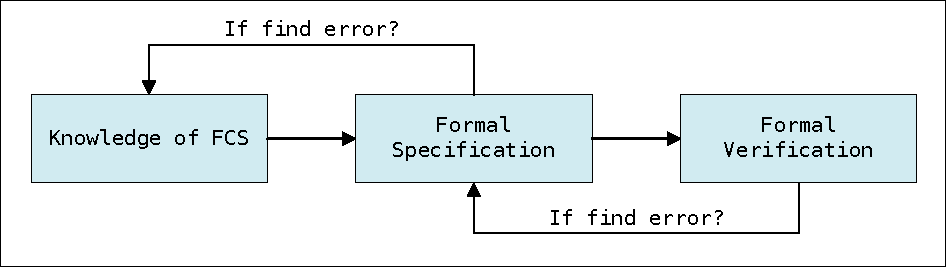
\includegraphics[width=1.0\textwidth]{knowledge_definition_proof.pdf}
\caption{A recursive procedure}
%\label{fig:label}
\end{figure}

\section{FML4FCS - Formal Method Library For Flight Control System in Coq}

\subsubsection{What is the FML4FCS}
It is an Formal Verification Library for Flight Control System (FML4FCS) developed under the COQ.
The Flight Control System (FCS) requires professional engineering knowledge in aerodynamics, electronmagnetism and mechanics, etc.
The algorithms in flight control are actually derived by using these knowledge or theories under many assumptions, and need lots of derivations.
We are not concerned with the correctness of these theories, but with the correctness of their derivation.

We made a simple division of the various types of people involved in the design of the flight control system.
(1) Domain Experts (ROLE - DE). The correctness of the theory should be left to the relevant experts.
(2) Formal Method Proof Engineer (ROLE - FMPE). The derivation is left to the formal method proof engineer.
(3) Computer Programmer (ROLE - CP). What programmers need is a reliable software repository that they can use.

This document is useful for all three types of people, but mainly for formal method proof engineers.

\subsubsection{How is the library organized}
This library is being built gradually, and organized by seperated sub-system at first stage.

For each subsystem, we follow the following steps:
\begin{enumerate}
\item Understand the engineering knowledge of the system and translate it into a mathematical document that suitable for formal verification.
Currently we only provide the English version mathematical document, other language versions need extra translation work.
\item Converts the mathematical document to COQ code and completes the proof of the lemma.
\item Use COQ's program extraction function to obtain reliable OCaml language library.
\item Presents some concrete sample programs so that users can observe and work with these work.
\end{enumerate}


%\newpage
% ++++++++++++++++++++++++++++++++++++++++++++++++++++++++++++++++++++++++++++++++++++++++++++++++++

\section{Sub systems of FCS}

The research object is flight control system of multicopter, especially an electric multi-rotor drone.
We started with subsystems tt the beginning.

\subsection{Propulsion System}
Propulsion system consists of four components: propeller, motor, electronic speed controller (ESC) and battery.
We modeled each of the components.

The main purpose of this section is to solve two kinds of problems, the forward solution and the reverse solution.

Forward solution refers to the estimation of performance indicators such as the longest hovering time, maximum load weight and maximum pitch angle of the aircraft when the parameters of each component are known.

Reverse solution refers to the design of the best parameters of each component under the required performance indicators.

We focus on the relatively simple forward issues, and the subsequent program will deal with the reverse issues.

\subsection{AttitudeSystem}

This part adds new mathematical theories, such as vectors, matrices, quaternions, etc.
Vectors and matrices are not available in COQ, we present an implementation.
We give an implementation of vectors, including the definitions of various operations and their properties.
The operations of vector, including addition, negative vector, subtraction, dot product, cross product, etc.

We define a matrix as a vector of a vector, and give the operations related to matrix and the transformation between vector and matrix, and give the proof of the properties of common operations.

Quaternions also have no library available in COQ, and we present several different implementations.
We have verified the multiplication formula of quaternions.
In addition, the quaternion is able to represent the rotation of the vector, and we have also tried to prove this theorem.
There are mainly three different methods of attitude representation, including Euler Angle, rotation matrix and quaternion.
Each of these three methods has its own advantages and disadvantages. 
Euler Angle is intuitive but has singularity; rotation matrix has no singularity but requires a large amount of computation when solving differential equations; although quaternions are not intuitive, they are not  singularity and have little computation.
Therefore, we will use these different methods interchangeably and need to convert between them.
We give the definitions of these transformation processes and attempt to give some proofs.


%\newpage
% ++++++++++++++++++++++++++++++++++++++++++++++++++++++++++++++++++++++++++++++++++++++++++++++++++
\section{The full system}



%\newpage
% ++++++++++++++++++++++++++++++++++++++++++++++++++++++++++++++++++++++++++++++++++++++++++++++++++
\section{Summary}
I think we've done the following:
1. Convert complex textual expertise in the field of flight control into a bottom-up verification and programming oriented reference manual.
It has built a unified dialogue bridge between field experts, verification engineers and software engineers, shielding the knowledge differences between people of different identities.
2. We have developed a working model. 
The domain expert only need to cares about the correctness of the presentation of the reference manual, and does not need to care about the correctness of the derivation and programming.
The verification engineer only needs to establish the build and verify the model and ensure the correct derivation according to the manual, and does not need to care about the theory and how to program;
Software engineers only need to use the manual to program, do not need to care about the theory and the correctness of these methods.
3. We have completed the formal verification of most subsystems in flight control.

In addition, our research method and part of the research results can also be used in other engineering fields.
Reliability is still the core task of future flight control system development. 
In addition, with the increase of system scale, development efficiency becomes more and more important.
Our goal is to design a development platform that automatically generates reliable software code for flight control applications.
This is done by first formalizing the system model, then configuring the system in a building block-like way, and finally using code generation tools to automatically generate the software.
Thus, we can ensure the reliability of the software, and improve the efficiency of software development.


\begin{thebibliography}{99}
\bibitem{qq} Quan Q. Introduction to multicopter design and control. Springer, 2017.
\end{thebibliography}

\end{document}